\section{Augstas jaudas pastiprinātājs}
No frekvenču augšuppārveidotāja signāla pievade notiek caur SMA konektoru, tad signāls tiek padots uz priekšpastiprinātāju KU PA 640720-10A\cite{pre_amplifier}, lai pastiprinātu ienākošo signālu par 30 dB. Priekšpastiprinātājam tiek nodrošināta jauda ar industriālā tipa barošanas avotu no 230 VAC uz 12 VDC. Tad +30 dBm signāls tiek nodots sadalītājam, kur uz katru kanālu tiek padota puse no ienākošās jaudas, kas ienākošo +27 dBm signālu pastiprina vēl par \textasciitilde19 dB katrs, kur tālāk +46 dBm signāls no katra kanāla tiek padots uz summatoru, pēc kā ir +\textasciitilde49 dBm, kur signāls tiek nogādāts uz nozarotāju, kur tālāk nogādāts N-tipa konektoram. Pie nozarotāja tiek pievienota jaudas monitorēšanas sistēma, lai noteiktu izstaroto un atstaroto jaudu. Darba punkta iestatīšanas un atiestatīšanas sistēma vajadzīga, lai nodrošinātu sistēmas drošu darbību.
HPA ir balstīts uz Qorvo QPM1017, kas darbojas vajadzīgajā augšupsaites joslā 7.145 līdz 7.235 GHz. Viens HPA modulis spēj nodrošināt līdz +50 dBm izejas jaudu ar 30… 40\% efektivitāti pie 7,2 GHz. Lai gan teorētiski viena moduļa izejas jauda ir +50 dBm, darba vadītājs nolēma apvienot divus QPM1017, kas ļautu katrai atsevišķai ierīcei darboties ar pusi no tās maksimālās jaudas, tādējādi uzlabojot termālo veiktspēju.
\begin{figure}[H]
	\centering
    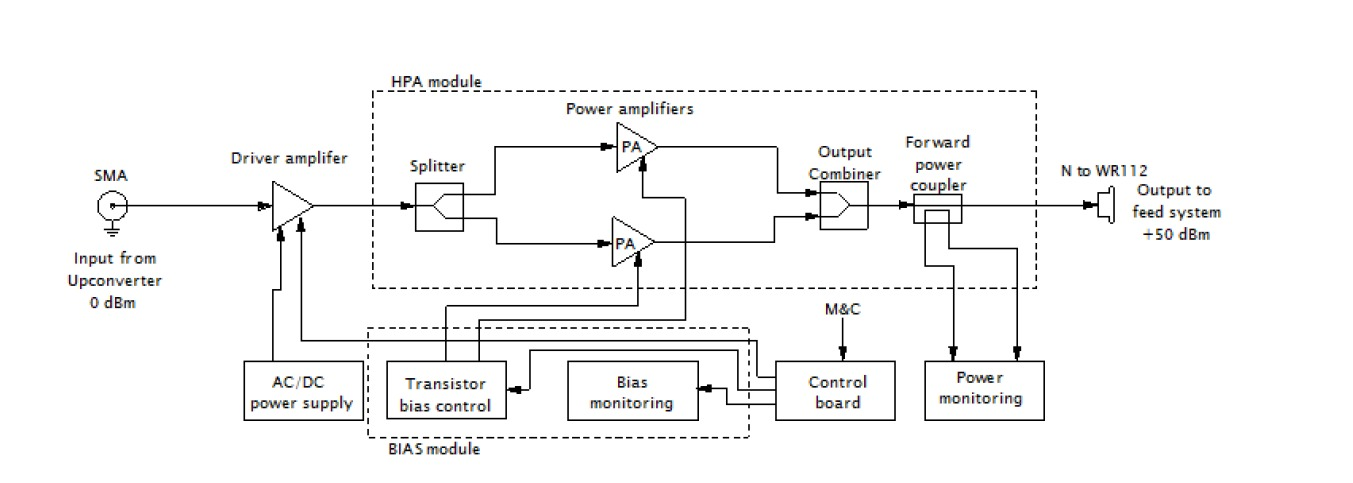
\includegraphics[width=0.9\textwidth]{pictures/HPA.jpg}\hspace{1cm}
    \caption{HPA vispārīga blokshēma \cite{bleideris2024xband}}
\end{figure}
1.3. att. var redzēt pašu jaudas pastiprinātāju ar ieejas filtriem. $V_{G}$ un $V_{D}$ ir pieslēgvietas, kuras ir jaudas pastiprinātāja vadībai un barošanas pievadei.
\begin{figure}[H]
	\centering
    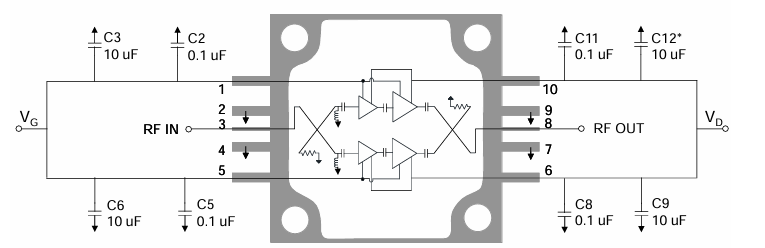
\includegraphics[width=0.9\textwidth]{pictures/pa.png}\hspace{1cm}
    \caption{QPM1017 sērijas RF jaudas pastiprinātājs}
\end{figure}
Šī darba ietvaros tiek izstrādāta darba punkta iestatīšana un atiestatīšanas sistēma, kas ir vadāma caur tīklu no kontroles datora, un jaudas monitoringa sistēma, kas mēra izstaroto un atstaroto jaudu.
